\chapter{Grundlagen}\label{chp:Grundlagen}
Im Folgenden soll ein \"Uberblick über die in dieser Arbeit verwendeten Technologien gegeben
werden. Eine allgemeine Einf\"uhrung in den Flugzeugentwurfsprozess zeigt anfangs die Einsatzgebiete des SGG-Editors auf.
Weiterhin wird auf das zentrale Datenformat CPACS, auf dem der SGG arbeitet, eingegangen und dessen Aufbau erl\"autert.
Im zweiten Teil werden die dargestellten Flugzeugkomponenten und verwendete Generierungsverfahren vorgestellt.

\section{Flugzeugentwurf}\label{sec:CPACS}
hier steht alles zum Flugzeugentwurfsprozess

\section{CPACS}\label{sec:CPACS}
Wie schon in Kapitel~\ref{sec:CPACS} beschrieben ... steht hier alles zu CPACS

\section{Profile}
Die Form des Querschnitts eines K\"orpers, wird im Folgenden als Profil bezeichnet. In der Aerodynamik ist die Entwicklung und Charakterisierung von Profilen ein wichtiges Teilgebiet. Konstruierte Profile sollen in ihrer Form bestimmten Funktionen gen\"ugen wie beispielsweise die Erzeugung eines dynamischem Auftriebs bei geringem Strömungswiderstand. In Cpacs wird zwischen Rumpf- und Tragfl\"achenprofilen unterschieden. Beide Profiltypen sind unter dem Konten \textit{profiles} als Listen f\"ur x, y und z Koordinaten repr\"asentiert.\\\\

	ooo hier steht ein tikz xml editor\\\\ 

\subsection{Fl\"ugelprofile}
hier steht allgemeines Zeug zu den Profilen

\newcounter{y}
\setcounter{y}{0}

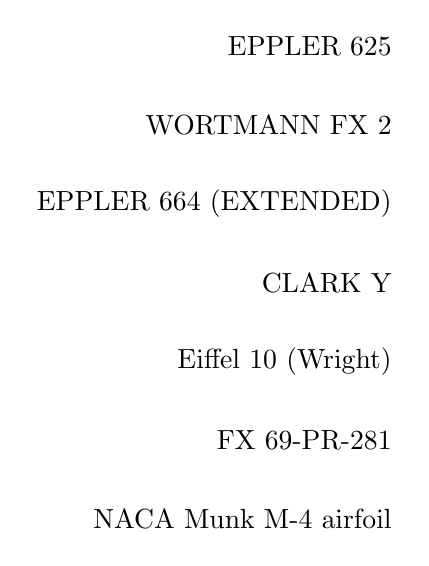
\begin{tikzpicture}
    \foreach \lbl / \fn in {EPPLER 625/e625.dat,
                            WORTMANN FX 2/fx2.dat,
                            EPPLER 664 (EXTENDED)/e664ex.dat,
                            CLARK Y/clarcy.dat,
                            Eiffel 10 (Wright)/eiffel10.dat,
                            FX 69-PR-281/fx69pr281.dat,
                            NACA Munk M-4 airfoil/m4.dat}{
        % Some profiles look better when using plot[smooth]
        \draw[yshift=-\arabic{y}cm,scale=3] node[left=0.5cm] {\lbl}
            plot file{tikz/data/\fn} -- cycle;
        \stepcounter{y}
    }  
\end{tikzpicture}
\footnotetext{Quelle: http://www.texample.net/tikz/examples/airfoil-profiles, Zugriff: 27.10.2014}


\subsubsection{NACA-Serie}
Das National Advisory Committee for Aeronautics oder kurz NACA wurde 1915 gegründet und ist ein direkter Vorg\"anger der US-Bundesbehörde für Luft- und Raumfahrt, NASA. Die NACA war eine amerikanische Organisation, die sich mit der Grundlagenforschung in der Luftfahrt beschäftigte. Eine bedeutende Entwicklung der NACA-Forschungen, sind optimierte Tragf\"achenprofile. Durch aerodynamischen Tests im Windkanal wurde bereits fr\"uh erkannt, dass die Fl\"ugelprofile mit den besten Eigenschaften hinsichtlich Auftriebsbeiwert und Widerstandsbeiwert, viele Gemeinsamkeiten besitzen. NACA-Profile sind somit Variationen eines Ursprungsprofils, die mit Hilfe von analytischen Gleichungen definiert werden. Spezifische Variationen dieses Profils werden durch die Kr\"ummung bzw. Steigung der Skelettlinie sowie die Dicke der Tragfl\"ache oberhalb und unterhalb jener Skelettlinie erzeugt. Im SGG-Editor wurde ein NACA-Generator implementiert, mit dem sich Profile der NACA 4-digit und NACA 5-digit Serie erstellen lassen.

\paragraph{Profile der Vierer-Serie}

In der vierstelligen NACA-Serie ist ein Profil definiert durch:
\begin{itemize}
\item[1.]Ziffer: maximale Profilw\"olbung 
	\begin{itemize}
		\item angegeben in Prozent, bezogen auf die L\"ange der Profilsehne
	\end{itemize}
\item[2.]Ziffer: W\"olbungsrücklage, Position der maximalen Profilw\"olbung
	\begin{itemize}
		\item angegeben in Zehnteln der L\"ange der Profilsehne
	\end{itemize}
\item[3./4.]Ziffer: maximale Profildicke
	\begin{itemize}
		\item angegeben in Prozent, bezogen auf die L\"ange der Profilsehne
	\end{itemize}
\end{itemize} 


Ein symmetrisches NACA 4 Profil kann mit Gleichung \ref{eq:symyt} konstruiert werden. Das Profil ist in seiner Form, nur durch die angegebene Profildicke ver\"andertbar, da die Profilw\"olbung und somit auch dessen Position die Werte Null haben. Gleichung \ref{eq:symyt} enth\"alt Konstanten, die f\"ur eine Profildicke von 20\% vorgesehen sind. Um diese Werte an die jeweils angegebene Profildicke anzupassen, wird die eigentliche Berechung mit $\frac{t}{0.2}$ multipliziert. In Gleichung \ref{eq:symyt} werden zus\"atzlich folgende Parameter verwendet:

\begin{itemize}
	\item[$c$ :] L\"ange der Profilsehne
	\item[$x$ :] Position entlang der Profilsehne auf der Abszissenachse von 0 to c, 
	\item[$y_t$ :] Entfernung der Skelettlinie zur jeweiligen Profilseite an Position x
	\item[$t$ :] Maximale Dicke des Profils multipliziert mit $\frac{1}{100}$
\end{itemize}

\begin{multline}\label{eq:symyt}
y_t= \frac{t}{0.2}c\left[0.2969 \sqrt{\frac{x}{c}} + (-0.1260) \left(\frac{x}{c}\right) + (-0.3516) \left(\frac{x}{c}\right)^2 + 0.2842 \left(\frac{x}{c}\right)^3 \right. \\\left. + (-1.015) \left(\frac{x}{c}\right)^4 \right]
\end{multline}


Soll die trailing edge geschlossen sein, also das Profil an dieser Position eine Dicke gleich Null haben, wird als Koeffizient an der letzen Stelle statt $-1.015$ ein Wert von $-0.1036$ gew\"ahlt.  Es ergeben sich folgende Definitionen f\"ur Ober- und Unterseite des Profils. Die x-Koordinaten sind f\"ur beide Seiten gleich, daher gilt $x_U = x_L = x$. Die y-Koordinaten ebenfalls identisch, nur das diese f\"ur die Oberseite positiv: $y_U = +y_t$ und f\"ur die Unterseite negativ sind: $y_L = -y_t$.\\
Die Generierung eines asymmetrischen NACA 4 Profils braucht zus\"atzlich zu Gleichung \ref{eq:symyt} noch die maximale Profilw\"olbung und die W\"olbungsr\"ucklage, also den Abstand der Profilnase zur maximalen Profilw\"olbung. 

\begin{itemize}
	\item[$m$ :] Maximale W\"olbung multipliziert mit $\frac{1}{100}$
	\item[$p$ :] Position der maximalen W\"olbung multipliziert mit $\frac{1}{10}$ 
	\item[$t$ :] Maximale Dicke des Profils multipliziert mit $\frac{1}{100}$	
\end{itemize}

Mit Gleichung \ref{eq:camber} wird die y-Koordinate der Skelettlinie an einer gegebenen x-Koordinate berechnet. 

\begin{equation}\label{eq:camber}
     y_c = \left\{ \begin{array}{ll} 
     					m \frac{x}{p^2} \left(2p - \frac{x}{c}\right), & 0 \leq x \leq pc \\[0.5cm]
         				m \frac{c-x}{(1-p)^2}\left(1+\frac{x}{c}-2p\right), & pc \leq x \leq c
         			\end{array}\right.
\end{equation}

\vspace{0.5cm}
Die Dicke des gekr\"ummten Fl\"ugelprofils ist senkrecht zur Skelettlinie festgelegt womit f�r Ober- und Unterseite des Profils folgendes gilt:

\begin{equation}
x_U = x - y_t \sin \theta \qquad , \qquad y_U = y_c + y_t \cos \theta
\end{equation}
\begin{equation}
x_L = x + y_t \sin \theta \qquad , \qquad y_L = y_c +-y_t \cos \theta
\end{equation}


$\theta = \arctan \left(\frac{dy_c}{dx}\right)$

\begin{equation}\label{eq:camber}
     \frac{dy_c}{dx} = \left\{ \begin{array}{ll} 
     					\frac{2m}{p^2} \left(p - \frac{x}{c}\right), & 0 \leq x \leq pc \\[0.5cm]
         				\frac{2m}{(1-p)^2}\left(p - \frac{x}{c}\right), & pc \leq x \leq c
         			\end{array}\right.
\end{equation}



text \cite{bib:naca_docu}
\subsubsection{Naca5}


\begin{equation}\label{eq:camber}
     y_c = \left\{ \begin{array}{ll} 
     					\frac{k_1}{6} \left\{x^3 - 3mx^2 + m^2 (3-m)x\right\}, & 0 \leq x \leq p \\[0.5cm]
         				\frac{k_1m^3}{6}\left(1-x\right), & p \leq x \leq 1
         			\end{array}\right.
\end{equation}



\begin{table}
\taburowcolors[2]{white .. black!20}
\centering
\sffamily\footnotesize
\tabulinesep=6pt
\begin{tabu}{|c|c|c|}
\hline
\rowcolor{RoyalBlue}\color{white}Position max W\"olbung (p) & \color{white}m & \color{white}k1\\
0.05 & 0.0580 & 361.400 \\
0.10 & 0.1260 &  51.640 \\
0.15 & 0.2025 &  15.957 \\
0.20 & 0.2900 &   6.643 \\
0.25 & 0.3910 &   3.230 \\
\hline
\end{tabu}
\caption{NACA 5 Konstanten f\"ur Auftriebskoeffizient von 0.3}
\end{table}


\subsubsection{Skelettlinie}
\begin{algorithm}[H]
 \KwData{bottom profile, top profile, trailing edge, leading edge}
 \KwResult{camber line }
 chord = line from trailing edge to leading edge\;
 \ForEach{p in chord}{
	perp1 = determine perpendicular of chord through point p\;
	\ForEach{p$\_$b in bottom profile}{
		perp2 = determine perpendicular of perp1 through point p$\_$b\;
		determine intersection point of perp1 and perp2\;
		determine distance from intersection point to p$\_$b\;
	}
	dist$\_$b = minimum distance from intersection point to p$\_$b\;
	\ForEach{p$\_$t in top profile}{
		perp2 = determine perpendicular of perp1 through point p$\_$t\;
		determine intersection point of perp1 and perp2\;
		determine distance from intersection point to p$\_$t\;
	}
	dist$\_$t = minimum distance from intersection point to p$\_$t\;	
	get center of dist$\_$t and dist$\_$b
 }
 \caption{Berechnung der Skelettlinie}
\end{algorithm}

\begin{figure}[htpb]
	\centering

\begin{tikzpicture}[scale=1.3]
\draw[dashed] (0,0)  -- (11,0) node[anchor=west] {};
\draw[] (7.0,-2) -- (7,3.5) node[anchor=south] {};
\draw[] (9.5,1.2) -- (1.0,1.2) node[anchor=south] {};
\draw[color=red] (1.9,1.2) circle (4pt);
\draw[color=red] (7.0,1.2) circle (4pt);
\draw (7.6,3.3) node {\scriptsize Normale 1};
\draw (4.0,1.0) node {\scriptsize Normale 2};

\draw (9.0,-0.2) node {\scriptsize Profilsehne};
\draw (1.7,1.45) node {\scriptsize p$\_$t};
\draw (7.75,0.9) node {\scriptsize Schnittpunkt};

% camber line    
\draw[smooth, scale=11] plot coordinates {(1.000000,-0.001260)(0.998459,-0.000891)(0.993844,0.000204)(0.986185,0.001995)(0.975528,0.004429)(0.961940,0.007435)(0.945503,0.010922)(0.926320,0.014786)(0.904508,0.018907)(0.880203,0.023155)(0.853553,0.027393)(0.824724,0.031479)(0.793893,0.035273)(0.761249,0.038641)(0.726995,0.041457)(0.691342,0.043611)(0.654508,0.045011)(0.616723,0.045586)(0.578217,0.045292)(0.539230,0.044113)(0.500000,0.042060)(0.460770,0.039175)(0.421783,0.035527)(0.383277,0.031213)(0.345492,0.026354)(0.308658,0.021088)(0.273005,0.015572)(0.238751,0.009973)(0.206107,0.004464)(0.175276,-0.000779)(0.146447,-0.005583)(0.119797,-0.009784)(0.095492,-0.013227)(0.073680,-0.015770)(0.054497,-0.017286)(0.038060,-0.017667)(0.024472,-0.016822)(0.013815,-0.014677)(0.006156,-0.011179)(0.001541,-0.006292)(0.000000,0.000000)(0.000000,0.000000)(0.001541,0.007462)(0.006156,0.015828)(0.013815,0.025031)(0.024472,0.034965)(0.038060,0.045492)(0.054497,0.056447)(0.073680,0.067641)(0.095492,0.078871)(0.119797,0.089923)(0.146447,0.100583)(0.175276,0.110640)(0.206107,0.119892)(0.238751,0.128156)(0.273005,0.135268)(0.308658,0.141087)(0.345492,0.145503)(0.383277,0.148432)(0.421783,0.149823)(0.460770,0.149656)(0.500000,0.147940)(0.539230,0.144718)(0.578217,0.140058)(0.616723,0.134060)(0.654508,0.126846)(0.691342,0.118564)(0.726995,0.109382)(0.761249,0.099488)(0.793893,0.089083)(0.824724,0.078383)(0.853553,0.067607)(0.880203,0.056983)(0.904508,0.046736)(0.926320,0.037085)(0.945503,0.028238)(0.961940,0.020390)(0.975528,0.013714)(0.986185,0.008359)(0.993844,0.004445)(0.998459,0.002061)(1.000000,0.001260)};    	
\end{tikzpicture}

	\caption{Berechnung eines Punktes der Skelettlinie}
	\label{fig:airfoil_chamber_algorithm}
\end{figure}



\subsubsection{Sonstiges}

\begin{figure}[htpb]
	\centering
\beginpgfgraphicnamed{profile-f1}
\footnotesize
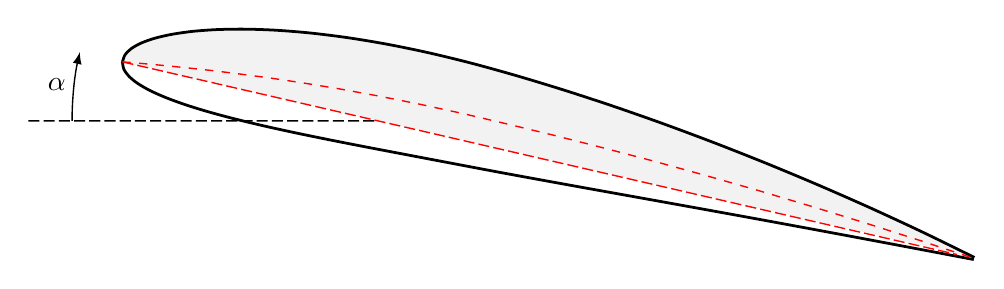
\begin{tikzpicture}[>=latex,scale=1.11]
\tikzstyle{spring}=[snake=zigzag,thick,line before snake=0.3cm,line after  snake=0.3cm,segment length=6,segment amplitude=5,join=round]%
\begin{scope}[rotate around={-13:(10,0)}]
% bottom_second
\draw[smooth,line width=1pt] plot coordinates {(0,0)(0.0334,-0.0767)(0.1087,-0.1437)(0.2253,-0.2011)(0.3824,-0.2489)(0.5790,-0.2870)(0.8139,-0.3158)(1.0860,-0.3355)(1.3940,-0.3466)(1.7365,-0.3497)(2.1123,-0.3457)(2.5199,-0.3356) (2.9580,-0.3209)(3.4252,-0.3029)(3.9198,-0.2835)(4.4427,-0.2625)(4.9936,-0.2377)(5.5666,-0.2102)(6.1594,-0.1810)(6.7696,-0.1513)(7.3950,-0.1217)(8.0332,-0.0930)(8.6815,-0.0653)(9.3376,-0.0386)(9.9988,-0.0125)};
% top_first
\draw[smooth,line width=1pt,fill=black!5] plot coordinates {(0,0)(0.0095,0.0831)(0.0624,0.1691)(0.1590,0.2574)(0.2990,0.3467)(0.4824,0.4357)(0.7085,0.5225)(0.9765,0.6050)(1.2855,0.6812)(1.6341,0.7488)(2.0206,0.8055)(2.4433,0.8492)(2.8998,0.8778)(3.3879,0.8897)(3.9049,0.8833)(4.4459,0.8592)(5.0064,0.8210)(5.5876,0.7687)(6.1870,0.7023)(6.8016,0.6219)(7.4286,0.5277)(8.0650,0.4197)(8.7080,0.2980)(9.3544,0.1623)(10.0012,0.0125)};
% sekelett
\draw[dashed, color=red, line width=0.5pt] plot coordinates { (0.0, 0.0)(0.021, 0.003)(0.086, 0.013)(0.192, 0.028)(0.341, 0.049)(0.531, 0.074)(0.761, 0.103)(1.031, 0.135)(1.34, 0.167)(1.685, 0.2)(2.066, 0.23)(2.482, 0.257)(2.929, 0.278)(3.407, 0.293)(3.912, 0.3)(4.444, 0.298)(5.0, 0.292)(5.577, 0.279)(6.173, 0.261)(6.786, 0.235)(7.412, 0.203)(8.049, 0.163)(8.695, 0.116)(9.346, 0.062)(10.0, 0.0) };
\draw[line width=0.5pt,dashed,dash pattern=on 4pt off 1.5pt,rotate around={13:(3,0)}](-1,0)--(3,0);
% arrows
\draw[line width=0.5pt,<-](3,0) +(180:3.5cm) arc (180:193:3.5cm);
\draw(3,0) +(186.5:3.7cm) node{$\alpha$};
% sehne
\draw[line width=0.5pt,color=red, dashed,dash pattern=on 4pt off 1.5pt](0,0)--(9.8,0);
\end{scope}%
\end{tikzpicture}
\endpgfgraphicnamed%



\begin{tikzpicture}
% profile with data file
%\newcounter{y}
\setcounter{y}{0}
\foreach \x in {1.00}
    \draw (11 cm,1pt) -- (11 cm,-1pt) node[anchor=north] {$\x$};
    \draw (1pt,0 cm) -- (-1pt,0 cm) node[anchor=east] {$0$};
	\draw (1pt,1.25 cm) -- (-1pt,1.25 cm) node[anchor=east] {$0.10$};
	\draw (1pt,-1.25 cm) -- (-1pt,-1.25 cm) node[anchor=east] {$-0.10$};
    \foreach \lbl / \fn in {naca4815.dat}{
        % Some profiles look better when using plot[smooth]
        \draw[yshift=-\arabic{y}cm,scale=11, fill=black!5]% node[left=0.5cm] {\lbl}
            plot file{tikz/data/\fn} -- cycle;
        \stepcounter{y}
    }
% axis
\draw[thick,-] (0,0)  -- (12,0) node[anchor=west] {x};
\draw[thick,-] (0,-2) -- (0,2) node[anchor=south] {y};    
% camber line    
\draw[smooth, dashed, scale=11] plot coordinates {(1.0,0.0)(0.998459,0.000614)(0.993844,0.0024245)(0.986185,0.0053355)(0.975528,0.00919)(0.96194,0.0137755)(0.945503,0.018829)(0.92632,0.0240435)(0.904508,0.029078)(0.880203,0.0335675)(0.853553,0.037132)(0.824724,0.039389)(0.793893,0.0399975)(0.761249,0.0399065)(0.726995,0.039667)(0.691342,0.039262)(0.654508,0.038677)(0.616723,0.037901)(0.578217,0.036926)(0.53923,0.03575)(0.5,0.034375)(0.46077,0.0328075)(0.421783,0.0310595)(0.383277,0.0291465)(0.345492,0.0270885)(0.308658,0.0249115)(0.273005,0.022642)(0.238751,0.0203125)(0.206107,0.0179555)(0.175276,0.0156075)(0.146447,0.013304)(0.119797,0.0110825)(0.095492,0.008979)(0.07368,0.0070285)(0.054497,0.005264)(0.03806,0.0037155)(0.024472,0.0024095)(0.013815,0.0013695)(0.006156,0.000613)(0.001541,0.000154)(0.0,0.0)};    	
\end{tikzpicture}    


\begin{tikzpicture}
% axis
\draw[thick,-] (11,0)  -- (12,0) node[anchor=west] {x};
\draw[thick,-] (0,-2) -- (0,2) node[anchor=south] {y};
% profile with data file
%\newcounter{y}
\setcounter{y}{0}
\foreach \x in {1.00}
    \draw (11 cm,1pt) -- (11 cm,-1pt) node[anchor=north] {$\x$};
    \draw (1pt,0 cm) -- (-1pt,0 cm) node[anchor=east] {$0$};
	\draw (1pt,1.25 cm) -- (-1pt,1.25 cm) node[anchor=east] {$0.10$};
	\draw (1pt,-1.25 cm) -- (-1pt,-1.25 cm) node[anchor=east] {$-0.10$};
    \foreach \lbl / \fn in {naca4815.dat}{
        % Some profiles look better when using plot[smooth]
        \draw[yshift=-\arabic{y}cm,scale=11]% node[left=0.5cm] {\lbl}
            plot file{tikz/data/\fn} -- cycle;
        \stepcounter{y}
    }
% camber line    
\draw[smooth, dashed, color=red, scale=11] plot coordinates {(1.0,0.0)(0.998459,0.000614)(0.993844,0.0024245)(0.986185,0.0053355)(0.975528,0.00919)(0.96194,0.0137755)(0.945503,0.018829)(0.92632,0.0240435)(0.904508,0.029078)(0.880203,0.0335675)(0.853553,0.037132)(0.824724,0.039389)(0.793893,0.0399975)(0.761249,0.0399065)(0.726995,0.039667)(0.691342,0.039262)(0.654508,0.038677)(0.616723,0.037901)(0.578217,0.036926)(0.53923,0.03575)(0.5,0.034375)(0.46077,0.0328075)(0.421783,0.0310595)(0.383277,0.0291465)(0.345492,0.0270885)(0.308658,0.0249115)(0.273005,0.022642)(0.238751,0.0203125)(0.206107,0.0179555)(0.175276,0.0156075)(0.146447,0.013304)(0.119797,0.0110825)(0.095492,0.008979)(0.07368,0.0070285)(0.054497,0.005264)(0.03806,0.0037155)(0.024472,0.0024095)(0.013815,0.0013695)(0.006156,0.000613)(0.001541,0.000154)(0.0,0.0)};  
% sehne
\draw[line width=0.5pt,color=red](0,0)--(11,0);    	
\end{tikzpicture} 
	\caption{Eine Vektorgrafik}
	\label{fig:vectorExample}
\end{figure}










\subsection{Rumpfprofile}
\blindtext





